%==========================================================================%
% MAIN PREAMBLE 
%==========================================================================%
\documentclass[12pt,letterpaper]{report}          % Single-sided printing for the library
%\documentclass[12pt,twoside]{report} % Double-sided printing
\usepackage[intlimits]{amsmath}
\usepackage{amsfonts,amssymb}
% \usepackage{gensymb}
\DeclareSymbolFontAlphabet{\mathbb}{AMSb}
%\usepackage{natbib}
\usepackage{float}
\usepackage[bf]{caption}       
\usepackage{fancyhdr}
%\usepackage{fancyheadings}
\usepackage{fancybox}
\usepackage{ifthen}
\usepackage{bu_ece_thesis}
\usepackage{url}
\usepackage{lscape,afterpage}
\usepackage{xspace}
\usepackage{epstopdf} 
\usepackage{subfig}
%==========================================================================%
%%% graphicx and pdf creation
\usepackage{graphicx}
\usepackage{appendix}
%\usepackage{psfrag}
%\DeclareGraphicsExtensions{.eps}   % extension for included graphics
%\usepackage{thumbpdf}              % thumbnails for ps2pdf
%\usepackage[ps2pdf,                % hyper-references for ps2pdf
%bookmarks=true,%                   % generate bookmarks ...
%bookmarksnumbered=true,%           % ... with numbers
%hypertexnames=false,%              % needed for correct links to figures !!!
%breaklinks=true,%                  % breaks lines, but links are very small
%linkbordercolor={0 0 1},%          % blue frames around links
%pdfborder={0 0 112.0}]{hyperref}%  % border-width of frames 
%                                   % will be multiplied with 0.009 by ps2pdf
%\hypersetup{
%  pdfauthor   = {Hasung Song <hwsong@bu.edu>},
%  pdftitle    = {dissertation.pdf},
%  pdfsubject  = {doctoral dissertations},
%  pdfkeywords = {mathematics, science, technology},
%  pdfcreator  = {LaTeX with hyperref package},
%  pdfproducer = {dvips + ps2pdf}
%}
%==========================================================================%
% customized commands can be placed here
%\newcommand{\figref}[1]{Figure~\ref{#1}}
%\newcommand{\chapref}[1]{Chapter~\ref{#1}}
%\newcommand{\latex}{\LaTeX\xspace}
%==========================================================================%
\usepackage[dvipsnames]{xcolor}
\usepackage{hyperref}
\hypersetup{breaklinks=true,colorlinks=true,linkcolor=blue,urlcolor=magenta,citecolor=cyan}
\usepackage{breakurl}
\usepackage{algorithm}

%==========================================================================%
% BEGIN
%==========================================================================%
\begin{document}

% \chapter{The KamLAND-ZEN Experiment}
\label{chapter:klz-detector}
\thispagestyle{myheadings}
\graphicspath{{2_Chapter_KLZ_Detector/Figures/}}

KamLAND, the \textbf{Kam}ioka \textbf{L}iquid-scintillator \textbf{A}nti Neutrino \textbf{D}etector, is a large liquid scintillator calorimeter detector situated 1km below mt. Ikenoyama in Gifu prefecture, Japan. I will describe the KamLAND detector's and the corresponding KamLAND experimental area's important components and features in this chapter. I will also explain how each component contributes to the KamLAND's scientific goals and the work of this thesis.


\section{KamLAND}
\label{sec:KamLAND}
One can think of KamLAND as an onion made up of many spherical layers, each layer serving the ultimate goal of shielding and observing the central core, the xenon-loaded liquid scintillator.


\subsection{Detector Infrastructure and Outer Detector}
The KamLAND detector is surrounded by the KamLAND experimental area, situated in an old iron mine, multiple caverns and passageways were excavated and set aside for KamLAND experimental use.

The KamLAND site is shown in Figure *. The control room contains networking and monitoring equipment which on-site shifters use to observe real-time detector activity. The first LS purification areas contain liquid-liquid extraction and nitrogen purge purification systems. The second LS purification area contains a distillation purification system. A new Xenon purification area was built for KamLAND-Zen. The dome area is a class 1,000 clean area atop the detector and includes a calibration source preparation room and electronics enclosure (electronics hut or e-hut). At the center of the dome area, there is a secondary class 100-1000 clean tent covering the KamLAND chimney. The inner balloon installations took place in August 2016 and May 2018 inside this clean tent.

The outer detector (OD) is a cylindrical water tank 20m tall and with 20m diameter and filled with pure water. The OD was refurbished in 2016, and 140 new 20-inch PMTs (R3600) were installed inside the cavity. The inner wall of the outer tank and the outer surface of the inner detector stainless steel spherical tank are covered highly reflective Tyvek sheets (Tyvek 1073B and 1082D) to collect as much of the light generated by crossing cosmic ray muons as possible. The outer detector's role is to tag cosmic ray muons, shield radioactivity and fast neutrons from the outer rock, and to stabilize the temperature of the ID.

\subsection{Inner Detector}
KamLAND's inner detector (ID) is the main spherical liquid scintillator detector, it is shown in Figure *. The ID is contained in a 18m diameter stainless steel sphere tank. 1,879 PMTs are mounted onto the inner wall of the ID, 1,325 17-inch and 554 20-inch PMTs. The PMTs are submerged in non-scintillating buffer oil (BO). An acrylic panel separates the buffer layer into two shells. This panel prevents the convection of radon out-gassed from PMT glasses into the central parts of the detector.

Photomultiplier tubes (PMTs) are KamLAND's eyes, detecting individual photons of light emitted by passage of particles through the scintillator volumes. Photons that hit PMT photocathodes are converted into a photoelectron. This photoelectron is then guided by electric fields to a series of dynodes. Each dynode multiplies the photoelectrons many times over, until the first photoelectron becomes $10^{6-7}$ electrons. Should multiple photons hit the photocathode simultaneously, the output voltage increases proportionally. This current is converted to a voltage by a coupling capacitor and read out via long coaxial cables. Figure ~\ref{fig:pmts} is a diagram of the 17in and 20in PMTs.

The 1,325 17-inch PMTs are Hamamatsu R7250s while the 554 20-inch PMTs are Hamamatsu R1449s and R3600s. The 20-inch PMTs were inherited from the Kamiokande experiment to increase our light collection. Both sets of PMTs have a bialkali photocathode sensitive to 300-650nm light which is well-suited for the emission spectrum of the LS. Figure ~\ref{fig:pmtqe} shows the quantum efficiency of the PMTs. The pmts also differ by dynode design; while the 17-inch PMTs feature "box-and-line" designs, the 20-inch PMTs have "venetian-blind styles". The different dynode designs along with the masking on the 17-inch PMTs, give us 17-in PMTs with better transit time spread (TTS) and 20-inch PMTs with better light collection efficiency. In total, the photocathode coverage of the ID is 34\%, with 23\% contributed by the 17-inch PMTs.

Furthermore, the PMT performance can be affected by the earth's magnetic field. To reduce this unwanted effect, the entire KamLAND detector is surrounded by geomagnetic compensation coils to counteract this external magnetic field. The residual magnetic field is less than 50mG, which has negligible effect on the PMT performance.

Another important characteristic of PMTs is their quantum efficiency (QE). The QE quantifies the probability that a photon arriving on the photocathode will produce a photoelectron. A PMT's QE varies over the wavelength of the incoming light. To improve our light collection, KamLAND's LS is doped with PPO to shift the wavelength of the incoming light to where the PMTs are most sensitive. Figure ~\ref{fig:qe_ppo} shows the PMT QE curve and the PPO reemission spectrum.

Next, is the 13m diameter outer balloon (OB). The OB is suspended in the center of the ID within the buffer oil, it is filled with one kiloton of highly purified organic liquid scintillator.

\subsection{Liquid Scintillator}
Liquid scintillator (LS) is the vital medium that sensitizes KamLAND to internal radioactivity. The KamLAND LS (KamLS), found in between the outer balloon and inner balloon, is composed of 80.2\% of dodecane (D12),1,2,4-trimethyl benzene, and 19.8\% pseudocumene (PC). A wavelength shifter called 2,5-diphenyloxazole (PPO) is added to the LS at a concentration of $1.36 \pm 0.03$ g/L. KamLAND-Zen has achieved $5 \times 10^{-18}$ g/g and $1.3 \times 10^{-17}$ g/g contamination for 238U and 232Th, respectively. The chemical composition of the KamLS can be found in Table ~\ref{tbl:kamls}

\begin{table}[h]
	\centering
	\renewcommand{\arraystretch}{1.2}
	\begin{tabular}{c|ccc}
		\hline
		& D12 & PC & PPO \\
		\hline
		Chemical Formula & C$_{12}$H$_{26}$ & C$_9$H$_{12}$ & C$_{15}$H$_{11}$NO \\
		Density [$g/cm^3$] & 0.7526 & 0.8796 & -\\
		Boiling Point [$^\circ$C] & 216 & 169 & 360 \\
		Melting Point [$^\circ$C] & -10 & -44 & 72 \\
		Flash Point [$^\circ$C] & 83 & 54 & - \\ \hline
	\end{tabular}
	\caption{Composition and properties of KamLAND Liquid Scintillator (KamLS)}
	\label{tbl:kamls}
\end{table}

\subsection{KamLAND-ZEN and XeLS}
At the center of KamLAND-ZEN lies the Xenon-loaded Liquid Scintillator (XeLS) contained in the 1.9m radius inner balloon (IB). The double-beta decaying isotope $^{136}Xe$ is thus placed in the cleanest, most sensitive part of the experiment. The Xenon gas is enriched to 90\% $^{136}Xe$ and is dissolved into a modified version of KamLS. The PPO concentration was increased to 4g/L to boost the light yield. This increased PPO concentration compensates for the 10\% reduction in emitted scintillation light when Xenon is mixed into the LS. The XeLS density is also tuned to match the surrounding KamLS. The chemical composition of the XeLS is shown in Table \ref{tbl:xels} in each of the different phases of the KamLAND-ZEN experiment.

\begin{table}[h]
	\centering
	\renewcommand{\arraystretch}{1.2}
	\begin{tabular}{c|cccc}
		\hline
		Material & Decane (\%) & PC (\%) & PPO (\%) & Xe (\%)\\ \hline
		Zen 400 Phase-1 & 82.3 & 17.7 & 2.7 & 2.44/2.48\\
		Zen 400 Phase-2 & 80.7 & 19.3 & 2.29$\pm$0.03 & 2.91\\
		Zen 800 & 82.4 & 17.6 & 2.38$\pm$0.02 & 3.13\\ \hline
	\end{tabular}
\end{table}

\section{Chemical Handling Infrastructure}

\section{Data Acquisition}

\section{KamLAND-ZEN Phases}

\subsection{KamLAND-ZEN 400}

\subsection{KamLAND-ZEN 800}

% Of course, there must be a Table of Contents, List of Figures and List of Tables at the beginning of the thesis, but this is all set up automatically.

{\bf Important}: You will also be using a lot of citations. The format in this template follows the so-called APA style and looks as follows in the document body: \cite{lamport1985:latex}, \cite{Debr01}. There are no numbers in the list of references -- the list is sorted alphabetically according to the first author's last name.

% Other styles of references are allowed by the library as well, e.g., ``plain'' or ``'ieee'', which use numbers in square brackets both in the document body and in the list of references. In order to use another style of references, e.g., ``plain'', follow the steps below:
% %
% \begin{enumerate}
%   \item In ``thesis.tex'' file:
% 	\begin{itemize}
% 	  \item comment out the line ``$\backslash$usepackage\{apalike\}'' at the top of the file,
% 	  \item replace ``$\backslash$bibliographystyle\{apalike\}'' with ``$\backslash$bibliographystyle\{plain\}'' towards the bottom of the file.
% 	\end{itemize}
%   \item In ``bu\_ece\_thesis.tex'' file, comment out all lines in the BIBLIOGRPAHY section (lines 503-517) and save it!
%   \item Recompile ``thesis.tex'' twice
% \end{enumerate}


% \cleardoublepage

\chapter{KamLAND-ZEN Simulation and Reconstruction}
\label{chapter:details}
\thispagestyle{myheadings}

\graphicspath{{3_Chapter_KLZ_Simulation_and_Reconstruction/Figures/}}

KamLAND-ZEN uses detailed simulations defined in KLG4Sim, a GEANT4-based Monte Carlo (MC) simulation software. The MC simulated events are tuned with real calibration events to carefully match real detector response. Simulated and physical events produce detector responses that are reconstructed to extract higher-level information such as energy and position. The reconstructed event information is used for data-selection and spectrum fitting. This chapter discusses the MC simulation and event reconstruction procedures used in KamLAND-ZEN 800.

\section{Analysis Framework}
\subsection{Data Flow}
Figure \ref{fig:dataflow} outlines the data flow in KamLAND-ZEN. PMT signals are digitized in either KamFEE or MoGURA, the two DAQ systems discussed in the previous chapter, the digitized signals are stored in Kinoko Data Format (KDF). KDF files contain trigger information and timestamped, digitized PMT waveforms. KDF files also store run condition information in the header. The EventBuilder collates the waveforms of a single event and stores them in a serial file. A waveform analyzer reconstructs a hit time and charge (TQ) information for each of these waveforms. The RTQ files hold the Raw-TQ information for each PMT. Event vertices and visible energy are derived from the RTQ files through their respective reconstruction algorithms. There are secondary reconstructions that are also applied to the RTQ files, such as muon track fitting, flasher vetos, double pulse fit, and unphysical event selections. The general vector file (GVF) is used for the main physics analyses like the one presented in this thesis.

\begin{figure}[htb]
	\centering
	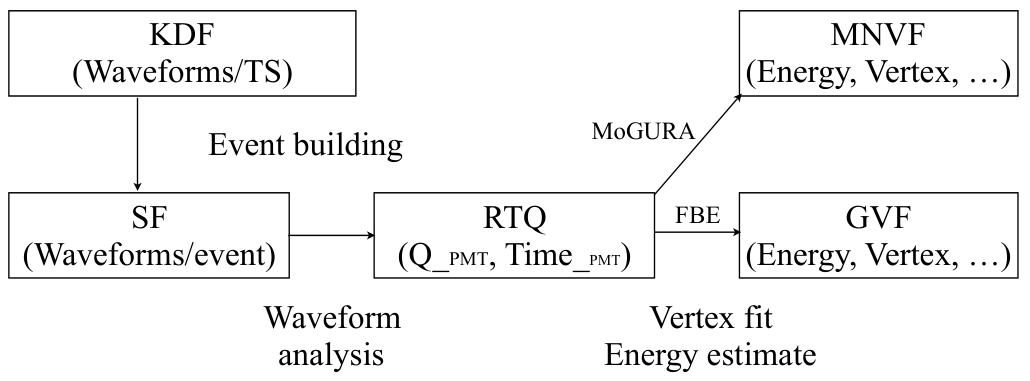
\includegraphics[scale=0.3]{dataflow.png}
	\caption{Data flow in KamLAND from raw waveforms to analysis variables such as energy, vertex, total hit PMTs, etc. \cite{ozaki_phd}}
	\label{fig:dataflow}
\end{figure}

GVF files contain the following information:
\begin{itemize}
	\item \textbf{run number}
	\item \textbf{event number}
	\item \textbf{TimeStamp} based on DAQ clock time (25 nsec for KamFEE, 20 nsec for MoGDAQ)
	\item \textbf{unixtime} is the number of seconds from January 1st in 1970 and used for some run vetos
	\item \textbf{trigger type} records which trigger was used
	\item \textbf{event vertex and badness} event vertices and a radius from detector center is saved, along with a vertex fit quality parameter called badness 
	\item \textbf{energy/energy17} visible energies given by the fitter, energy17 is the energy estimate only using 17-inch PMTs
	\item \textbf{TotalChargeID/17/OD} sum of all PMT charges of each PMT type
	\item \textbf{numhit/numhit17} the number of hit PMTs/17-inch PMTs in each event.
	\item \textbf{NsumMax} a maximum number of hit PMTs in a single DAQ cycle within each event, a "peak" nhit of the event
	\item \textbf{N200OD} Maximum number of simultaneous hit OD pmts within 200nsec windows
	\item \textbf{muon entrance and direction} muon fitter results are recorded.
\end{itemize}

Finally, MoGURA events are associated with muon events acquired in KamFEE DAQ (FBE) and stored in a Muon-Neutron Vector File (MNVF) to search for neutron capture events that occur shortly after muons.

\section{Event Reconstruction}
\subsection{Waveform Analysis}
Each digitized waveform has 128 samples with 1.5ns sample times; this corresponds to a waveform digitization window of 192 ns. The waveforms are processed and TQ reconstructed with the following procedure.
\begin{itemize}
	\item \textbf{Smoothing} Each waveform is smoothed via a running-average first derivate.
	\item \textbf{Baseline adjustment} The baseline of each PMT is collected at the beginning of each run. This baseline is subtracted from each waveform.
	\item \textbf{Peak finding} Peaks are found with running-averaged 1st, 2nd, and 3rd derivatives.
	\item \textbf{Leading-edge and Trailing-edge tag} A leading-edge is stamped as 10ns before the peak voltage. The trailing edge is stamped when the waveform returns to baseline. An example of this time-stamping is shown in Figure \ref{fig:waveform_analysis}
	\item \textbf{Waveform Sum calculation} The waveform is integrated from the leading-edge to the trailing-edge.
\end{itemize}

\begin{figure}[htb]
	\centering
	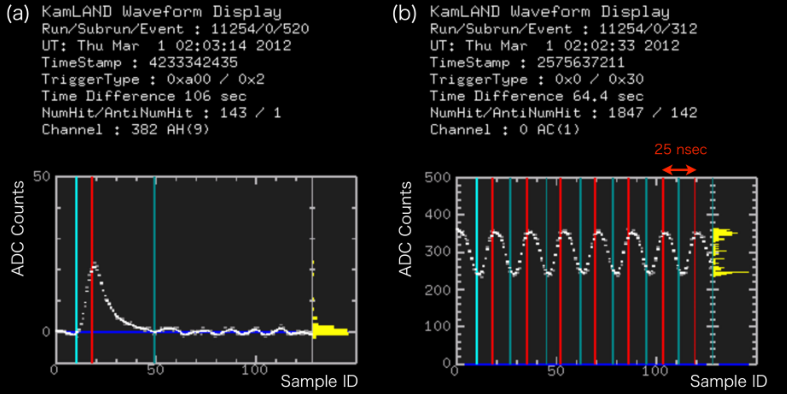
\includegraphics[scale=0.5]{waveform_analysis.png}
	\caption{An example of waveform analysis from thesis \cite{yoshida_phd}. (left) ADC counts of a real waveform after baseline subtraction. The left cyan line is the leading edge, the center red line is the peak position, and the right dark cyan line is a trailing-edge. (right) Clock calibration example on 25 nsec intervals.}
	\label{fig:waveform_analysis}
\end{figure}

When there are mulitple hits in one PMT waveform, the total charge of the hits and the earliest hit time is returned. This simplified information is used for the vertex and energy reconstruction. The multi-pe information is used for a double-pulse fit and a muon shower tag.

\subsection{PMT Corrections}
\subsection*{Low Gain Problem and HV Reductions}
Since ~2011, we observed that the gain of some of the 17-inch PMTs gradually decreased. As the gain of the PMTs fell, this compormises signal/background ratio and PMT waveform quality. It was also observed that the PMTs enter a low impedance state before the gain dropped. A HV current and voltage monitor allows for the real-time monitoring of this state. Usually a simple HV power cycle could recover normal PMT behavior. Since 2016, a auto HV power cycle mechanism was implemented to mitigate the low gain problem, but the root case is still unknown.

Each time the PMTs enter the low impedance state, the HV on that channel was reduced in 50-100 V increments. Over time, some of the channels had their HV reduced by 450 V. FIgure \ref{fig:lowgain_trend} shows the trend in low gain 17-inch PMTs.

\begin{figure}[htb]
	\centering
	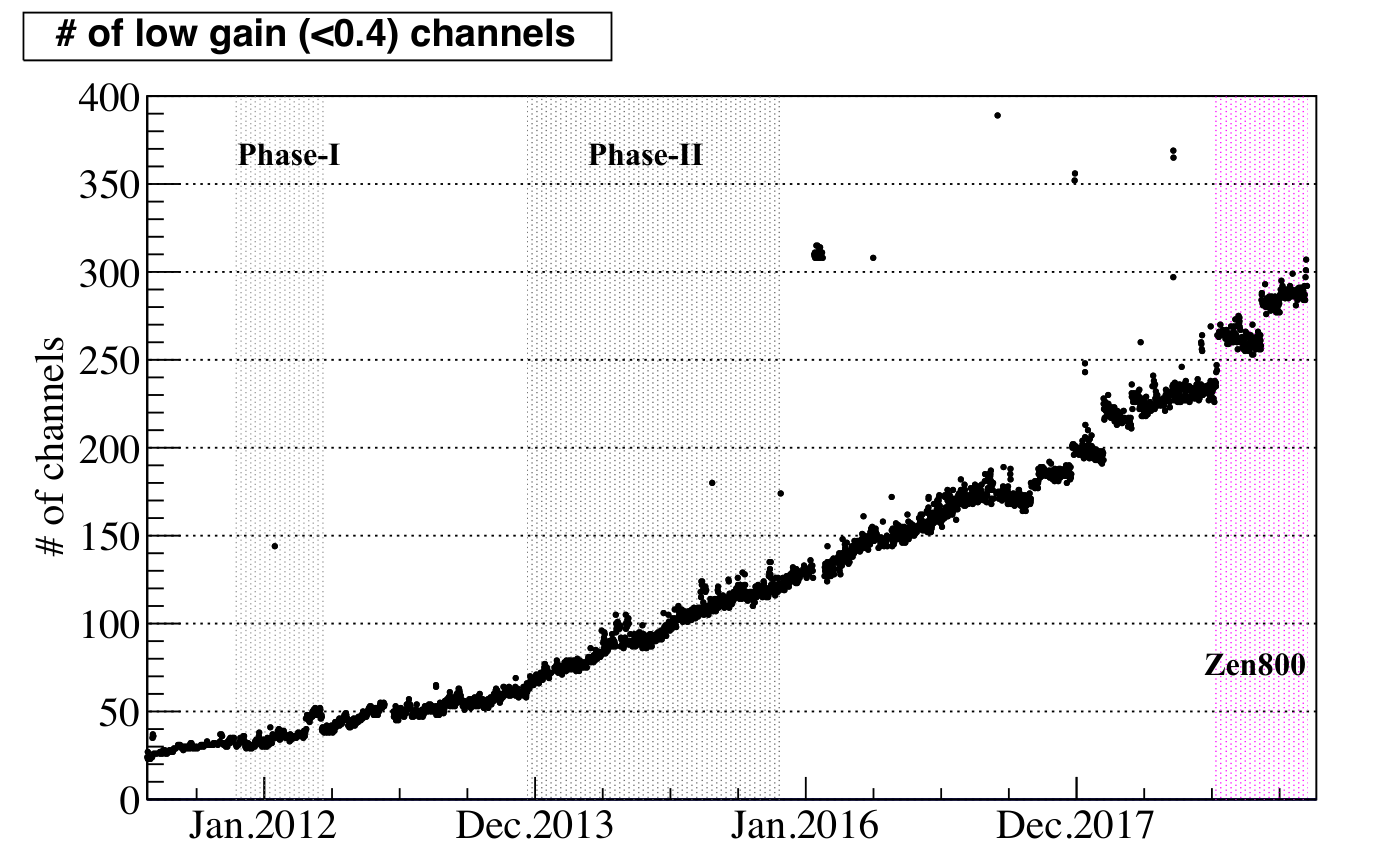
\includegraphics[scale=0.3]{lowgain_trend.png}
	\caption{The trend in the number of low gain 17-inch PMTs, before ZEN-800. The number of low gain channels increased gradually, while the sudden increases are from HV reductions performed since 2017 \cite{ozaki_phd}.}
	\label{fig:lowgain_trend}
\end{figure}

%/ TODO
Note about current low pmt gain analysis.

\subsection*{Bad Channel}
A channels is considered bad if the PMT meets one or more of the following criteria:
\begin{itemize}
	\item PMT pulses less than 0.6\% of the time over all events
	\item PMT pulses below 0.48\% for non-muon events
	\item PMT pulses less than 80\% of the time for high-energy muon events
	\item PMT is missing a waveform more than 10\% of the time
	\item Large discrepancy between the two ATWD hits
	\item High muon charge PMTs. A PMT may read much higher charge ($Q_{detected}$) than the average of its surrounding PMTs ($Q_{expected}$). A run is divided into 100 muon intervals, for each interval the criteria is defined as
	\[\frac{1}{N_{interval}}\sum_{i=1}^{N_{interval}}\left(\frac{1}{N_{muon}}\sum_{j=1}^{N_{muon}}\frac{(Q_{expected}-Q_{detected})^2}{Q_{expected}}\right)>1000\ p.e.\]
\end{itemize}
These bad channels are excluded from event reconstruction and physics analyses.

\subsection*{Dark Hit}
Thermal fluctuations can emit electrons off the photocathode leading to a PMT hit signal. These "dark hits" are an unavoidable hit-level background in PMT detectors, lowering the detector temperature reduces this effect. The dark hit rates are measured from run-to-run and are factored into our likelihood-maximizing reconstruction algorithms. The hit rate observed 50-100 ns before the PMT hittime rising edge is taken as the dark rate, Figure \ref{fig:darkrate} shows the PMT hittime distribution and the dark rate window.

\begin{figure}[htb]
	\centering
	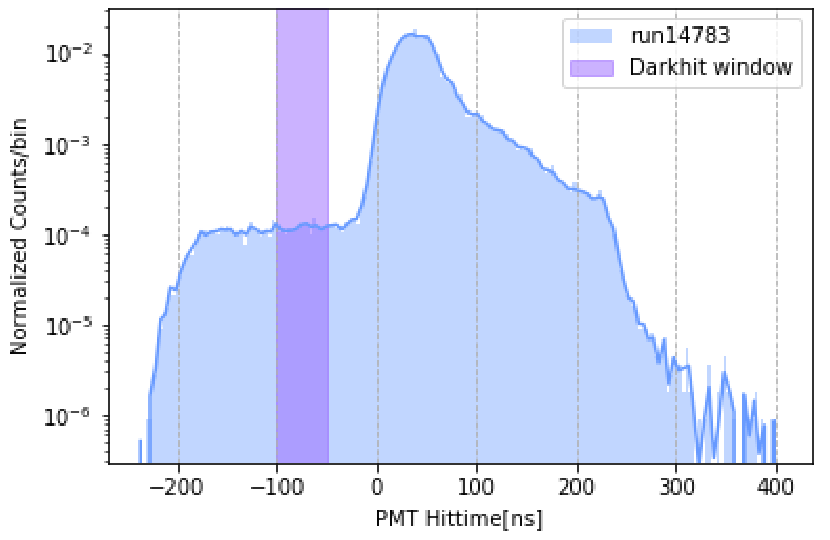
\includegraphics[scale=0.4]{darkrate.png}
	\caption{An example pmt hit time distribution from data run 14783, the 50-100 ns leading window is taken to measure the pmt dark hit rate. \cite{li_phd}.}
	\label{fig:darkrate}
\end{figure}

\subsection{Primary Vertex Fitter}
The primary vertex fitter provides a rough estimate of a scintillating event's location. This estimate serves as the input to a more thorough, but complex secondary fitter. The fit works by constructing a hit time residual distribution:
\begin{equation}
	T_{i}^{emit}=T_i-TOF_i = T_i - \frac{\left|R_i-r_{vertex}\right|}{c_eff}
	\label{eq:prim_vertex}
\end{equation}
Here $T_i$ is the hit time of the $i^{th}$ PMT, $TOF_i$ is the time it takes for a scintillation photon to traverse from the vertex position to the $i^{th}$ PMT position, $R_i$ is the PMT position, $r_{vertex}$ is the unknown vertex position to fit for, and $c_{eff}$ is the speed of light in the given medium. By fitting $T_i^{emit}$ to match the standard scintillation time profile, a primary $r_{vertex}$ is produced by the fitter.

\subsection{Secondary Fitter}
The secondary V2 fitter uses the $r_{vertex}$ given by the primary fitter to compute $T_0$ according to the equation \ref{eq:sec_v2}
\begin{equation}
	T_0 = \frac{\sum_i \left(T_i^{pmt}-TOF^{pmt}_i\right)\times Q_i}{\sum_iQ_i}- const.
	\label{eq:sec_v2}
\end{equation}
\begin{figure}[htb]
	\centering
	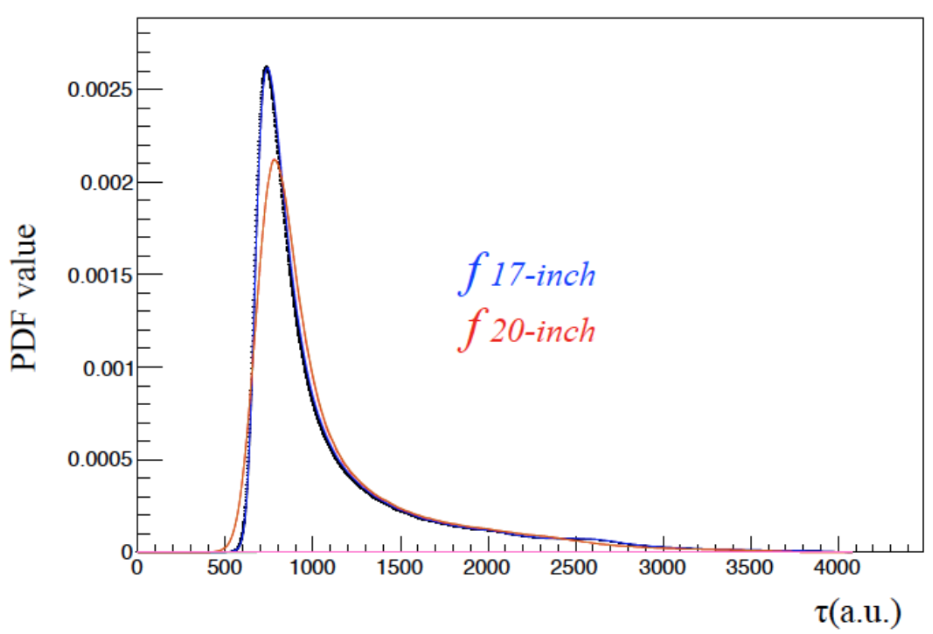
\includegraphics[scale=0.4]{pmt_dist.png}
	\caption{Probability density function of 17-inch and 20-inch PMT hit times calculated from calibration data. The plot is from \cite{ozaki_phd} and originally from a 2005 calibration dataset.}
	\label{fig:pmt_pdfs}
\end{figure}
This $T_0$ is the charge weighted sum of $T_emit$ from \ref{eq:prim_vertex}. This $T_0$ serves as the universal start point of an event. From this time, each pmt hit time is
\begin{equation}
	\tau(x,y,z,T_0) = T^{pomt}_i-TOF_i^{pmt}-T_0
\end{equation}
Finally, these time-of-flight corrected and centered hit time distributions are used to create probability distributions for the 17 and 20 inch PMTs respectively. These PDFs are shown in Figure \ref{fig:pmt_pdfs}. The likelihood function for an individual PMT is defined as:
\begin{equation}
	\phi_i =\frac{\mu\times f_i(\tau_i)+D_i}{\mu\times C_{17/20}+D_i}
\end{equation}
Here, $\mu$ is the pulse shape determination factor, $D_i$ is the dark hit rate for the $i^{th}$ PMT and $C_{17/20}$ is the normalization constant for the 17 or 20 inch PMTs. The overall log-likelihood is given by the $log(L)=\sum_ilog(\phi_i)$. The log-likelihood is maximized by the Newton-Raphson method, in which the $x,y,z,T_0$ are adjusted to the best-fit values, giving us the V2 reconstructed vertex.

\subsection{Energy Reconstruction}
Likelihood maximization is also used to reconstruct the energy of an event. A likelihood PDF is constructed using the number of hits, charge, and hit timing.
\subsection*{$N_{hit}$ PDF}
The expectation of the number of photons hitting PMT i, $\mu_i$ is a function of the visible energy and dark charge.
\begin{equation}
	\mu_i = a_i(x,y,z)\times E_{vis} +d_i
\end{equation}
Here, $a_i(x,y,z)$ is a coefficient that converts the event energy to the number of photons which is calibrated with the neutron events. It is determined by the PMT position $x,y,z$. $d_i$ is the dark noise charge of PMT i, which is electronically measured. The probability that $\mu_i$ photons hit the $i$th PMT $j$ times, $k_{ij}$, is ideally expressed by the poisson distribution:
\begin{equation}
	k_{ij}=\frac{(\mu_i)^j}{j!}e^{-\mu}
\end{equation}

However, in KamLAND waveform analysis, the 1 p.e. detection efficiency is reduced by the 0.3 p.e. software charge threshold. This threshold is set to reduce the acceptance of dark noise but also decreases hit detection efficiency. As a result, the PMT hit probablity is reduced to:
\begin{equation}
	P_{hit}=1-v_ie^{-\mu_i}
\end{equation}

\subsection*{Hit Charge PDF}
A Gaussian distribution is assumed for the hit charge PDF of each PMT:
\begin{equation}
	f_{i,j(q_i)}=\frac{1}{\sqrt{2\pi j\sigma^2}}exp(-\frac{(q_i-j)^2}{2j\sigma^2})
\end{equation}
$q_i$ is the observed charge in p.e. units and $\sigma$ is  the charge resolution against 1 p.e. distribution.

\subsection*{Hit Time PDF}
PMT hit timing factors into energy reconstruction by helping to discriminate hits unrelated to the physical event. The hit timing model is created using source calibration data. 
\begin{equation}
	P_{time,i} = \frac{\psi(t_i)a_i E_{vis}+d_i}{\mu_i}
\end{equation}
The PDF is the sum of the signal hit distribution and the constant dark noise.
\subsection*{Energy Likelihood}
The likelihood function to be maximized is constructed as 
\begin{equation}
	L=\prod_{Not\ hit\ PMTs}P_{no-hit,i}\prod_{Hit\ PMTs}\left[P_{hit,i}\left(\sum_{j=1}^{100}f_{i,j}\right)P_{time, i}\right]
	\label{eq:energy_likelihood}
\end{equation}
The reconstructed energy is the one which maximizes this likelihood. The Newton-Raphson method is used to search for this energy. This process is implemented independently for the 17-inch PMTs and 20-inc PMTs, then the event energy is calculated with a weighting factor $\alpha$:
\begin{equation}
	E_{vis}=(1-\alpha)E_{17inch}+\alpha E_{20inch}
\end{equation}
The weighting factor $\alpha=0.3$ was determined to maximizing energy resolution.
\subsection{Bad Channels in Energy Reconstruction}
The increase in the number of low gain PMTs has lead to worsening energy resolution over time, as these PMTs are excluded from the typical energy reconstruction described above. In particular, some of the low gain PMTs still detect photons, but proper gain calibration is not possible. A method for utilizing the information from operational low gain PMTs was developed, and the basic strategy is as follows:
\begin{enumerate}
	\item The change in gain causes the effect of the 0.3 p.e. threshold on hit probability to change. The no-hit probability was expanded as follows:
	\begin{equation}
		P^{\prime}_{no-hit, i} = \left(1+\epsilon_1\mu_i+\epsilon_2\frac{\mu_i^2}{2!}+\epsilon_3\frac{\mu_i^3}{3!}\right)e^{-\lambda\mu_i}
	\end{equation}
	This model was originally a simple expansion of $P_{no-hit}$, but in the end was adjusted phenomologically to better reproduce real data. This adjustment is why an additional $e^{-\lambda\mu}$ appears in the model.
	\item The parameters $\epsilon_1, epsilon_2, epsilon_3,$ and $\lambda$ are estimated with actual data. The events satisfying the following selections are collected and the no-hit probability is calcualted for each expected charge. The expected charge of the i-th PMT $\mu_i$ is estimated using the vertex and total charge of the events that meet the following conditions.
	\begin{itemize}
		\item $r<6m$
		\item Not muons or events within 2 ms after muons
		\item Events with more than 120 17-inch PMT hits
		\item PMT waveforms that contain only 1 peak
	\end{itemize}
	Figure \ref{fig:nohit_prob} shows the result of fitting this adjusted no-hit probability model. THe fitting is performed run-by-run and for each PMT independently.
	\item Use the updated no-hit probability pdf in the event energy reconstruction in Equation \ref{eq:energy_likelihood}.
\end{enumerate}
\begin{figure}[htb]
	\centering
	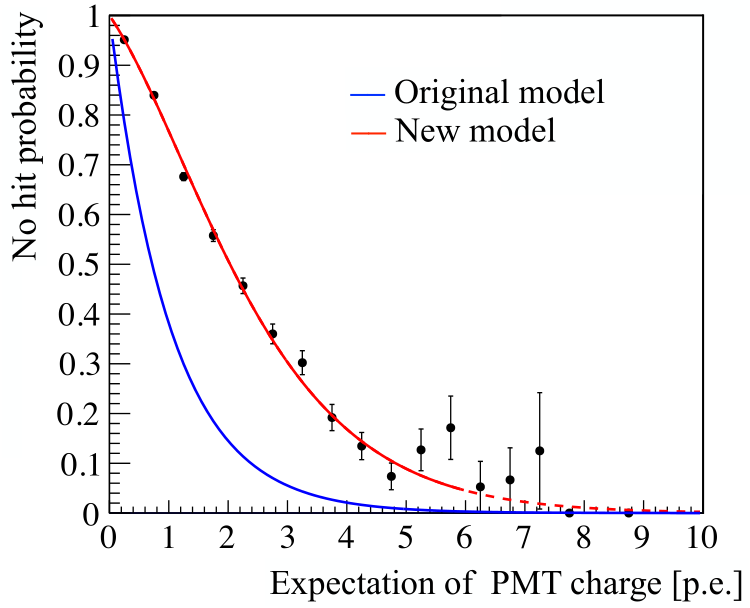
\includegraphics[scale=0.4]{no-hitprob.png}
	\caption{Fitting no hit probability to a low gain PMT against the expected charge $\mu$. The original model is shown with the blue line while the red line is the new model which agrees better with low-gain PMT data.}
	\label{fig:nohit_prob}
\end{figure}

Making use of the low-gain PMTs can improve energy resolution by up to 3\% \cite{karino_master}. Further analysis in this work uses energy reconstructed from the combination of normal and low-gain PMTs.

\subsection{Muon Reconstruction}
The selection and understanding of muon and muon-correlated neutrons are essential to multiple background rejections. This section, describes the special selection criteria and reconstruction methods used for muons and neutrons.
\subsection*{Muon Selectrion Criteria}
The muon event selection criteria are as follows:
\begin{itemize}
	\item Total charge of 17inch PMTs, $Q_{17}\geq 10000$ p.e.
	\item $Q_{17geq}$ 500 p.e. and the number of hit OD PMTS $\geq 9$.
\end{itemize}
The former criteria selects muons which go through the scintillator volumes of the detector. A total charge of 10,000 p.e. roughly corresponds to an event energy of 30 MeV, which exceeds the energy range of most physical analyses in KamLAND-ZEN. The second selection is for muons that only deposit energy in the outer buffer oil (clipping muons). Muons passing through the buffer oil volumes do not scintillate, as such the 500 p.e. threshold in Chrenkov radiation roughly corresponds to about 40 MeV of energy deposition.
\subsection{Cosmic Ray Muon Reconstruction}
Cosmic ray muon events form tracks as opposed to the point-like events caused by single decay events. The process is shown diagramattically in Figure \ref{fig:muon_reco}
\begin{enumerate}
	\item The ID PMT which detects the earliest light is identified. If the charge of this hit is low or isolated in time from the many other hits in the event, it is classed as a dark hit and ignored. A line is drawn from the earliest hit muon PMT and the center of the KamLAND detector. The intersection of this line and the outer balloon is marked as the temporary entrance point.
	\item The PMT whose charge is the largest is identified. The brightest hit PMT should be hit later than the earliest PMT and the neighbors of the earliest PMTs. A line is drawn from the brightest hit PMT and the center of the KamLAND detector. The intersection of this line and the outer balloon is marked as the temporary exit.
	\item The temporary track is defined as the line connecting the temporary entrance and exit. The temporary track is finally corrected by checking the correlation between the track length and the total charge.
	\item The reconstruction quality is evaluated by checking the following:
	\begin{itemize}
		\item Whether the earliest and the brightest PMTs can be identified
		\item Whether the mean hit time of PMTs around the entrance is earlier than the around the exit.
	\end{itemize}
	A "badness" parameter value is assigned to the reconstruction according to this evaluation. With this evaluation, around 15\% of muon candidates are regarded as badly reconstructed though they can still be used in muon-neutron pairing. Bad muon reconstruction is caused by ringing in the PMT signals, muon bundles, and stopped muons.
\end{enumerate}
\begin{figure}[htb]
	\centering
	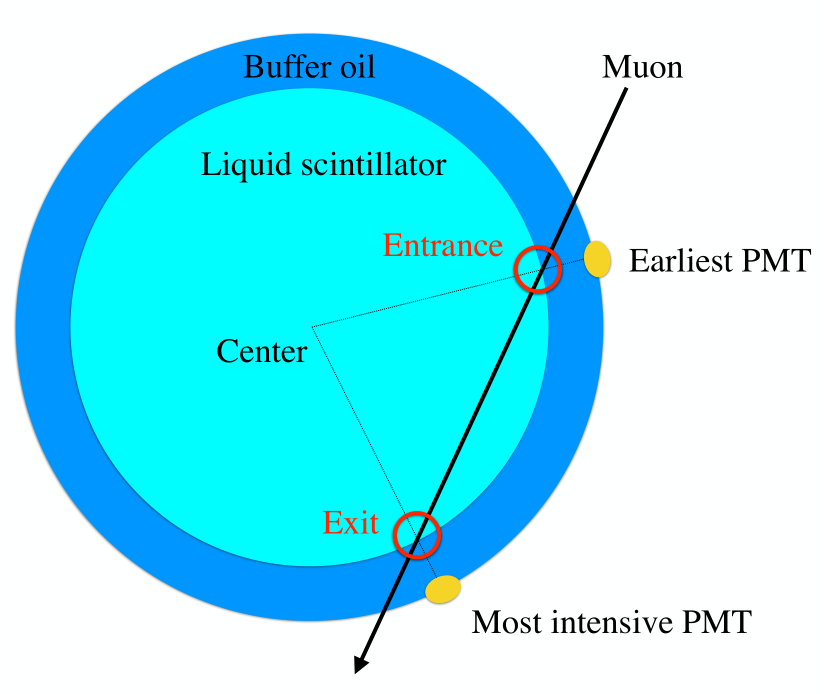
\includegraphics[scale=0.4]{muon_reco.png}
	\caption{A schematic of muon track reconstruction in KamLAND.}
	\label{fig:muon_reco}
\end{figure}
The light yields in the muon events are estimated in :
\begin{equation}
	\langle dQ_C/dX\rangle =28\pm 5\textbf{p.e./cm (Cherenkov muons)}
\end{equation}
\begin{equation}
	\langle dQ_S/dX\rangle =338\pm 12\textbf{p.e./cm (Scintillation muons)}
\end{equation}
\subsection{MoGURA Neutron Reconstruction}

\section{Event Selection}



%==========================================================================%
% Bibliography
\newpage
\singlespace
\bibliographystyle{plain}

% each subdirectory can have its own BiBTeX file
\bibliography{thesis} % same bib file as main thesis
\cleardoublepage

%==========================================================================%
% Curriculum Vitae
% \phantomsection\addcontentsline{toc}{chapter}{Curriculum Vitae}

\begin{center}
    {\LARGE \bf CURRICULUM VITAE}\\[0.5in]
    {\large \bf Hasung Song}\\[0.1in]
    Department of Physics\\
    Boston University\\
    Email: hwsong@bu.edu\\
    % Add more contact info as needed
\end{center}

\vspace{0.3in}

\section*{Education}
\begin{itemize}[leftmargin=*]
    \item \textbf{Ph.D. in Physics}, Boston University, 2019--Present
    \item \textbf{M.Sc. in Physics}, Boston University, 2019--2022
    \item \textbf{B.Sc. in Physics}, University of California, Berkeley, 2016-2018
\end{itemize}

\section*{Professional Experience}
\begin{itemize}[leftmargin=*]
    \item \textbf{Post-Baccalaureate Researcher}, University of California, Berkeley, 2018--2019
\end{itemize}

\section*{Selected Publications}
\begin{itemize}[leftmargin=*]
	\item "Search for Majorana Neutrinos with the Complete KamLAND-Zen Dataset" KamLAND-Zen Collaboration,	arXiv:2406.11438 [hep-ex] (2024)
	\item "Eos: conceptual design for a demonstrator of hybrid optical detector technology" T. Anderson et al. JINST 18 P02009 (2023)
	\item "KamNet: An integrated spatiotemporal deep neural network for rare event searches in KamLAND-Zen" A. Li, et al. Phys. Rev. C 107, 014323 (2023)
	\item "RFSoC-based front-end electronics for pulse detection" S.N. Axani et al. 2024 JINST 19 P03013 (2024)
	\item "Search for the Majorana Nature of Neutrinos in the Inverted Mass Ordering Region with KamLAND-Zen" KamLAND-Zen Collaboration, Phys. Rev. Lett. 130, 051801 (2023)
\end{itemize}

\section*{Scientific Collaborations}
\begin{itemize}[leftmargin=*]
	\item EoS Collaboration 2023--Present
	\item NuDOT Collaboration 2022--Present
    \item KamLAND Collaboration 2020--Present
    \item NIM+ 2020--2021
	\item Mu2E Collaboration 2018--2019
\end{itemize}

\section*{Conferences and Presentations}
\begin{itemize}[leftmargin=*]
    \item "Getting Excited About Double Beta Decay in KamLAND-Zen", APS DNP, Talk, Boston, MA, 2024.
    \item "Understanding KamNet Performance in KamLAND-ZEN with ML Interpretability", SLAC Summer Institute, Poster, SLAC, 2023.
    \item "KamLAND-Zen's New ML Tricks", Neutrino Physics and Machine Learning, Talk, Northeastern University, 2023.
    \item "Rejecting Spallation Backgrounds in KamLAND-ZEN with KamNet", Neutrino, Poster, Seoul, Korea, 2022.
    \item "Rejecting Spallation Backgrounds in KamLAND-ZEN with KamNet", TAUP, Poster, Valenica, Spain, 2021.
    \item "Neutrinoless Muon-to-Positron Conversion at Mu2e", APS April Meeting, Talk, Denver, Colorado, 2019.
\end{itemize}

\section*{Teaching Experience}
\begin{itemize}[leftmargin=*]
    \item Physics 211 General Physics I, Teaching Assistant, Boston University, Summer 2020.
    \item Physics 211 General Physics I, Teaching Assistant, Boston University, Fall 2019.
\end{itemize}

\section*{Professional Service}
\begin{itemize}[leftmargin=*]
    \item Member, Graduate Student Council, Boston University Physics Department, 2019--Present.
\end{itemize}

\end{document}
 

%==========================================================================%
\end{document}
